\section*{Introduction}

DNA double-strand breaks (DSBs) pose a serious threat to the integrity of bacterial cells. They can arise from various sources such as gamma radiation\cite{Krasin1977}, antibiotic exposure, or collision of the replication fork with DNA-bound proteins\cite{Dillingham2008}. In \emph{E. coli}, DSB repair is initiated by the RecBCD complex. However, different sources of DSBs can lead to different repair pathways, as illustrated on Figure \ref{Fig:DSB_scheme}.

% Two-sided DSBs
In the case of a two-sided DSB (Figure \ref{Fig:DSB_scheme}A), created for example by radiation or antibiotics, the double-stranded DNA (dsDNA) ends are first recognised by the RecBCD complex, which will translocate along the DNA at a speed of $\sim$1.6 kb/s, thanks to its combined 5' and 3' helicase activities\cite{Wiktor2018}. While translocating, RecBCD will digest both DNA strands until it meets a specific 8-base pair sequence (5'-GCTGGTGG-3') called Chi-site. Upon recognition of the Chi-site, RecBCD will pause briefly before resuming translocation, albeit with modified nuclease activity: the 5' DNA end will be degraded more slowly, and the 3' end will not be degraded at all, leading to a 3' DNA overhang. Of note, Chi recognition by RecBCD is not systematic, and was previously reported to occur with $\sim$40\% probability by an \emph{in-vitro studies}\cite{Taylor1992}. As RecBCD creates the 3' overhang, the nuclease domain of its RecB subunit will promote loading of the RecA protein onto the single-stranded DNA (ssDNA)\cite{Churchill2000, Spies2006}. The resulting RecA-DNA nucleoprotein filament will be used as a template to search for an intact homologous sequence and perform homologous recombination. It is still unclear at which point exactly RecBCD dissociates from the DNA and what specificly triggers the dissociation. One \emph{in-vitro} study suggested that RecBCD dissociation was triggered by Chi recognition\cite{Taylor1999}, but the RecA filament could also play a role.

% Fork reversals
Another frequent cause of DSB formation in \emph{E. coli} is the collision of the replication fork with DNA-bound proteins (Figure \ref{Fig:DSB_scheme}B), which has been reported to occur in $\sim$18\% of cells per cell cycle\cite{Sinha2018} and leads to the disassembly of the replisome\cite{Michel1997}. The resulting Y-shaped DNA structure is bound by the RuvAB complex, which will pull the DNA strands (in a process called "branch migration") to create a "chicken-foot" four-way DNA structure\cite{Seigneur1998}. The free end of this structure (DNA tail) is bound by RecBCD, which will either (i) digest the whole DNA tail and displace RuvAB, allowing the replisome to be re-loaded, or (ii) recognise a Chi-site and load the RecA protein onto the 3' end of the DNA tail\cite{Michel2001}. Since this part of the DNA was recently replicated, a homologous sequence is necessarily present in close proximity, and can be used for homologous recombination.

In the case of fork collisions, the DSB repair process is expected to occur faster than in the case of a two-sided break caused by antibiotics or radiation. Since the DNA tail is only a few kilobases long, its full digestion by RecBCD would only take a few seconds, and if a Chi-site is recognised and RecA loaded, the close proximity of a homologous sequence should ensure rapid homology searching ($\sim$1.5 min)\cite{Amarh2018}. In the case of a two-sided break however the homologous sequence is not guaranteed to be nearby, and the homology search can take close to 10 min\cite{Wiktor2021}.

\begin{figure*}[htbp]
    \centering
    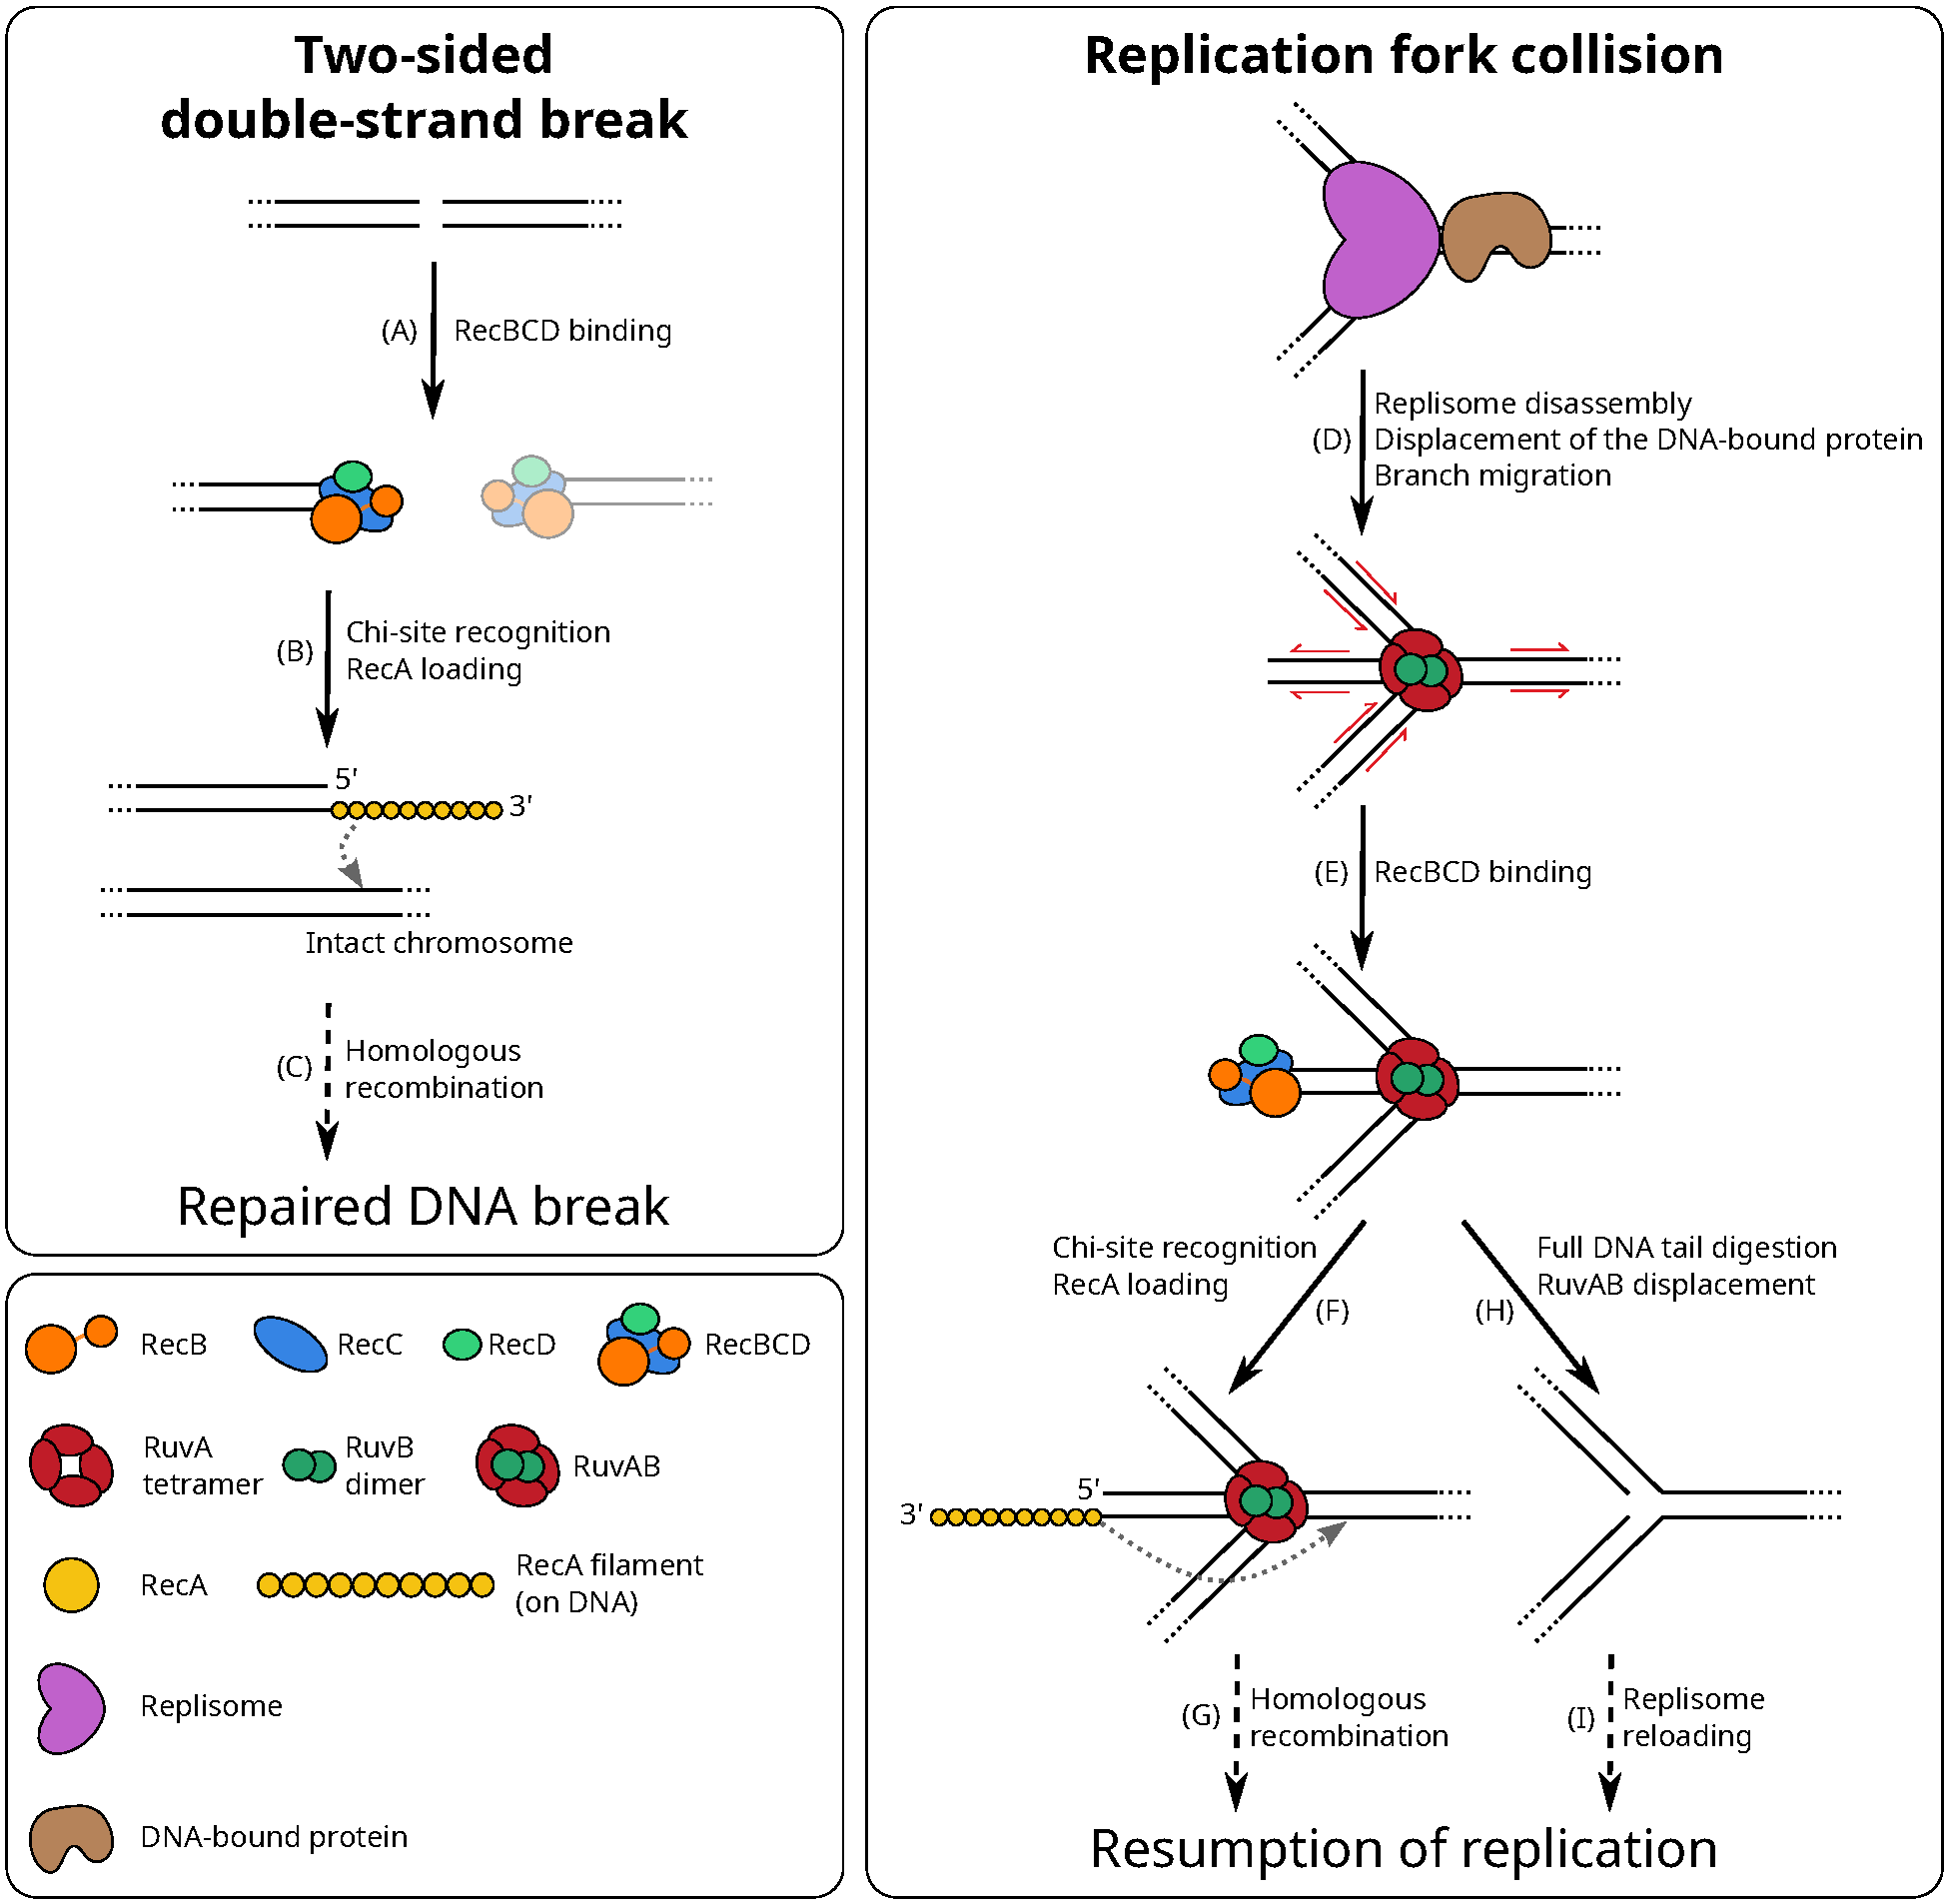
\includegraphics[width=.8\textwidth]{Figures/DSB_scheme.pdf}
    \caption{Double-strand break repair by RecBCD in \emph{E. coli}. \textbf{Left}: two-sided DSB. \textbf{(A)} RecBCD binds to both free dsDNA ends. \textbf{(B)} RecB translocates along the DNA, while digesting both the 5' and 3' strands. Upon recognition of a Chi-site, RecBCD stops degrading the 3' strand, and loads the RecA protein onto it. \textbf{(C)} After a homologous sequence has been found for the RecA-coated ssDNA, homologous recombination leads to two intact copies of the DNA. \textbf{Right}: replication fork collision. \textbf{(D)} The collision of the replisome with a DNA-bound protein leads to replisome disassembly. The RuvAB complex binds to the DNA junction, and performs branch migration. \textbf{(E)} RecBCD binds to the free dsDNA end and degrades both DNA strands. \textbf{(F)} RecBCD recognises a Chi-site, stops degrading the 3' strand, and loads RecA onto it. \textbf{(G)} The four-way DNA structure is resolved by homologous recombination and DNA replication can resume. \textbf{(H)} Alternatively, RecBCD digests the whole dsDNA tail to the junction and displaces RuvAB. \textbf{(I)} The replisome is re-loaded, and DNA replication can resume.}
    \label{Fig:DSB_scheme}
\end{figure*}

% Mutants in the repair pathway
Mutants in the repair pathway will deal differently with these types of damage. Cells that are \emph{recA}-deficient (\dreca) will be entirely unable to repair two-sided DSBs, and the prolonged action of RecBCD on the DNA will result in the digestion of large parts of the chromosome\cite{Horii1968, Chow2007}. \emph{recA}-deficient cells are however capable of repairing DSBs arising from fork reversal, thanks to RecBCD's exonuclease activity (Figure \ref{Fig:DSB_scheme}B, reaction G)\cite{Seigneur1998, Michel2001}. The $D_{1080} \rightarrow A$ point mutation in the RecB subunit of the RecBCD complex (\teneighty) abolishes RecB's nuclease activity, as well as its ability to load the RecA protein on DNA\cite{Yu1998, Wang2000}. The other activities of the complex (DSB recognition, DNA unwinding, Chi-recognition) are unaffected\cite{Anderson1999}. Despite the loss of its RecA loading activity, the \teneighty\ mutant is still able to repair two-sided DSBs. \teneighty CD will unwind DNA at the break without degrading it, and the Single-Strand Binding protein (SSB) will coat the 3' ssDNA, while the RecJ exonuclease degrades the 5' ssDNA. Finally, the RecFOR complex will displace SSB and load RecA, allowing for homologous recombination to occur\cite{Ivancic-Bace_2003}. This process should allow the \teneighty\ mutant to repair both two-sided DSBs and DSBs generated through replication fork collision, albeit at a slower rate. Of note, a \dreca-\teneighty double-mutant, which lacks both the RecA protein and RecB's nuclease activity, would be entirely unable to repair both types of DSBs.

% Ciprofloxacin
Ciprofloxacin is an antibiotic of the fluor\-quinolones family, which causes DSBs. Im \emph{E. coli}, it does so by binding covalently to DNA topoisomerase II (gyrase), and trapping it in a DNA-bound conformation\cite{Kohanski2010}. Even though it is known that ciprofloxacin creates DSBs that are repaired by RecBCD, the exact mechanism through which the DSBs are created is still unclear. Since the poisoned gyrase is tightly bound to DNA, it is likely to cause replication fork collisions\cite{Wentzell2000, Drlica2008}, and the subsequent repair of a chicken foot structure (Figure \ref{Fig:DSB_scheme}B). Furthermore, the ciprofloxacin-poisoned gyrase is trapped in the "open" stage of its catalytic cycle, where it holds together two disjointed DNA ends. Therefore, upon removal of the gyrase (through a process that involves the ExoVII nuclease\cite{Huang2021}), we can reasonably expect the formation of a two-sided DSB. This is supported by previous observations that ciprofloxacin can cause DSBs independently of DNA replication\cite{Zhao2006}. Taken together, these results suggest that in fast-growing cells, which contain multiple replication forks, both replication-dependent and independent DSBs occur.

% Overview of the article
In this study, we aimed to learn more about the repair of ciprofloxacin-induced DSBs by RecBCD. We took advantage of RecBCD's low copy number ($\sim$5 molecules per cell on average\cite{Lepore2019a}) to perform enhanced localisation microscopy\cite{Yu2006, Elf2007} using a fully functional fusion of RecB to the Halo-tag that was previously developed and tested in the lab\cite{Lepore2019a}. This allowed us to detect and localise DNA-bound RecB molecules \emph{in-vivo}, and to estimate how long RecBCD stays bound to DNA. By exposing cells to different ciprofloxacin concentrations during imaging, we were able to look at the evolution of the repair process over time, and assess how cells were coping with different levels of DNA damage. To broaden our view of the repair process, we imaged a fluorescent fusion to the RecA protein in the same conditions. Finally, imaging RecB in the \dreca, \teneighty\ and \dreca-\teneighty\ mutants gave us insight into the factors that might affect RecBCD's dissociation from the DNA.
